\documentclass[12pt]{article}
\usepackage{nott-titlepage}
\usepackage{graphicx}
\usepackage{float}
\usepackage{siunitx}
\usepackage{listings}

\title{Performance of a PMSM Part 1}
\author{Tan Hong Kai}
\date{November 19 2023}
\studentid{20386501}
\module{EEEE3114 Electrical Machines, Drive Systems and Applications}
\department{Department of Electrical and Electronics Engineering}

\begin{document}
\maketitle

\section{Introduction}

A permanent magnet synchronous motor (PMSM) is simulated in FEMM software. The motor is given in a DXF file. However, a modified version of the model is used throughout the simulations conducted using an anti-periodic air gap in FEMM to increase the simulation speeds. A few simulations were conducted in a series of tasks to explore the characteristics of the motor. To further automate the changing of parameters in the model, the FEMM \textbf{MATLAB} interface were used to collect the data and plot it.

The motor has a rated speed of 1500 rpm with 4 poles (2 pole pairs). It has a rated current of $20$ A peak to peak. The peak torque is at $\ang{90}$ load angle. Each of the poles have 6 slots, each current phase have 2 windings. 

\section{Task 1}

The first task is to explore the cogging torque generated by the motor in no load conditions. Three different values were noted about the cogging torque. The first value is the torque ripple frequency/period. The other two values are the maximum and minimum torque of the torque ripple. 

\subsection{Methodology}\label{task-1-method}

The cogging torque is the torque generated on the rotor due to the preferred rotor alignment at no load. This can be measured in FEMM by changing the rotor orientation around the windings and measuring the torque. The rotor orientation can be changed by changing the inner angle in the air gap parameters for the anti-periodic air gap. A loop is used to iterate through all the angle and the torque obtained by measuring the gap integral of the anti-periodic air gap.

The ripple frequency can be calculated using the \lstinline{fft} function in MATLAB and double-checked visually on the plot. The maximum and minimum can be taken from the data using \lstinline{max} and \lstinline{max} function.

\subsection{Results}

\begin{figure}[H]
    \centering
    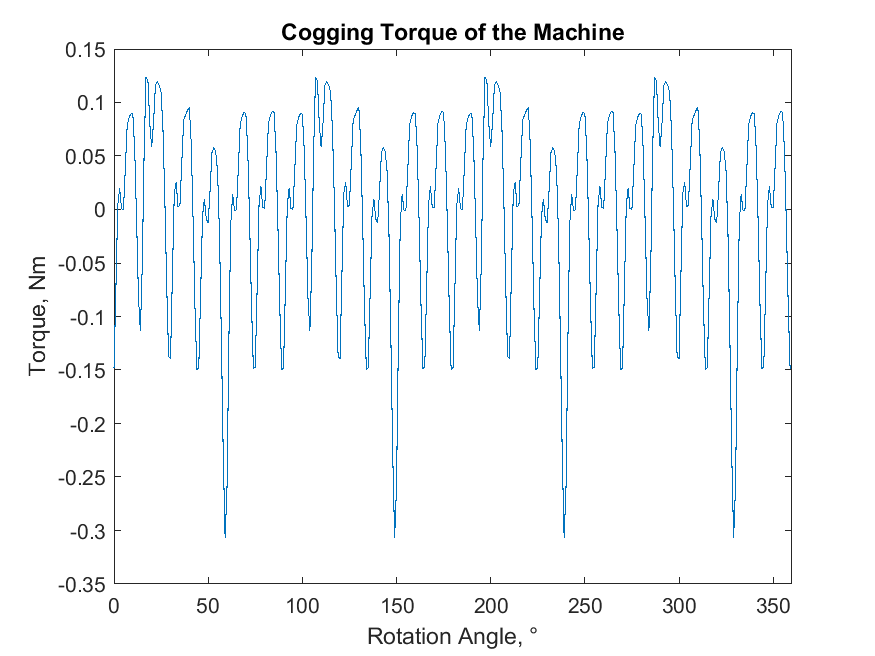
\includegraphics[width=\linewidth]{img/task_1.png}
    \caption{Cogging Torque of the Machine}
    \label{fig:task-1}
\end{figure}

\subsection{Analysis}

The measured cogging torque period is $\ang{15}$ (24 pulsations per revolution). This is due to the windings of the stator in the motor. When the rotor rotates, the permanent magnet induced current in the windings at no load, which oppose the motion of the rotor. Since there are a total of 24 slots in the model, the opposing torque will have a period of $\frac{\ang{360}}{24} = \ang{15}$.

The maximum torque ripple is $0.1240$ Nm while the minimum torque $-0.3068$ Nm. This makes the maximum cogging torque magnitude $0.3068$ Nm.

\section{Task 2}

The second task is to explore and plot the back EMF generated by the machine. The machine constant is then calculated from the back EMF using equation \ref{eq:back-emf}, where $E_{b}$ is the back EMF, $K_{m}$ is the machine constant and $\omega_{r}$ is the rated mechanical speed.

\begin{equation}\label{eq:back-emf}
    E_{b} = K_{m} \omega_{r}
\end{equation}

\subsection{Methodology}

The back EMF of the motor can be calculated using equation \ref{eq:back-emf-flux}. $d\phi$ is the change in flux induced in the winding, This can be calculated using the \lstinline{diff} function. $dt$ is the time period between the flux change and $E_{b}$ is the back EMF.

\begin{equation}\label{eq:back-emf-flux}
    E_{b} = \frac{d\phi}{dt}
\end{equation}

To obtain the transient differences, the rotor is rotated for one full rotation and measuring the flux in all the windings. The difference between the measured flux is calculated. The $dt$ can be calculated using the rated speed of the motor. The maximum back EMF magnitude is used for the machine constant calculation.

\subsection{Results}

\begin{figure}[H]
    \centering
    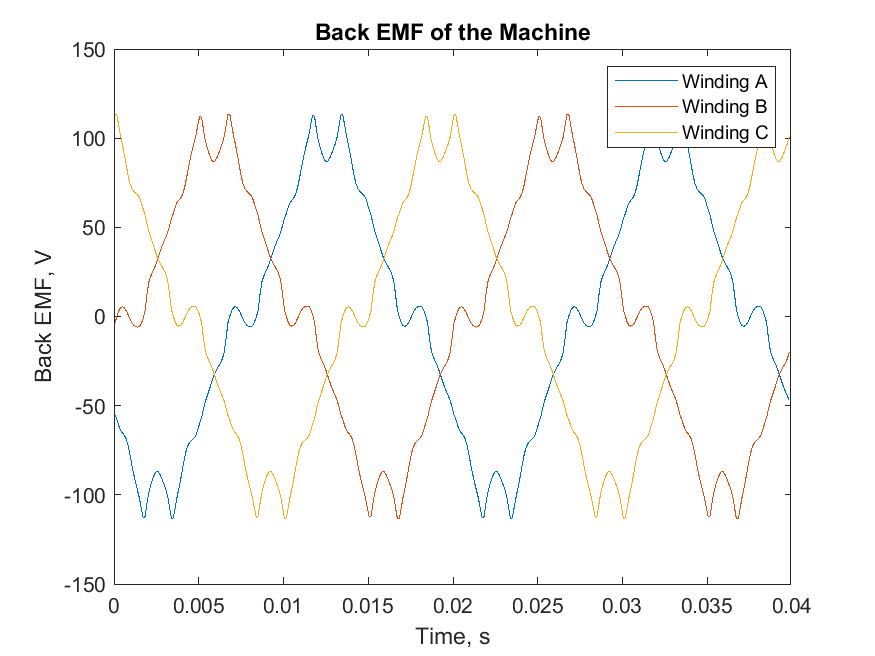
\includegraphics[width=1\linewidth]{img/task_2_1.png}
    \caption{Back EMF Across all Rotor Angles}
    \label{fig:task-2}
\end{figure}

\subsection{Analysis}

The peak back EMF generated by the machine is $113.1587$ V. At $1500$ rpm, $\omega_{r} = 1500 * \frac{2\pi}{60} = 157.0796$ rad/s. Using the back EMF $K_{m} = \frac{113.1587}{157.0796} = 0.7204$.

\section{Task 3}

The third task is to explore the rated torque (mean torque) developed at different load angles. The resultant torque ripple frequency and magnitude is also simulated and analysed.

\subsection{Methodology} \label{task-3-method}

At different rotation of the rotor, the torque developed is different at the same load angle. A quick simulation is set up to get the initial rotor angle with $0$ Nm and maximum torque generated. This can be done by having a fix load angle at rated current and rotate the rotor (see \ref{task-1-method}).

To explore the rated torque at different load angle, the rotor is rotated to minimum torque angle. The circuit property is then modified with different load angle and the torque developed is measured.

The torque ripple of the machine can be obtained by starting with rotor angle at maximum torque magnitude. To ensure the rotor stays at maximum torque, the rotor is also rotated at half the speed ($\ang{0.5}$).

The frequency of the ripple can be obtained by performing FFT, while the ripple magnitude can be calculated by subtracting the maximum torque with the minimum torque. The maximum and minimum can be obtained using \lstinline{max} and \lstinline{min} function. The mean torque is calculated using the \lstinline{mean} function.

\subsection{Results}

\begin{figure}[H]
    \centering
    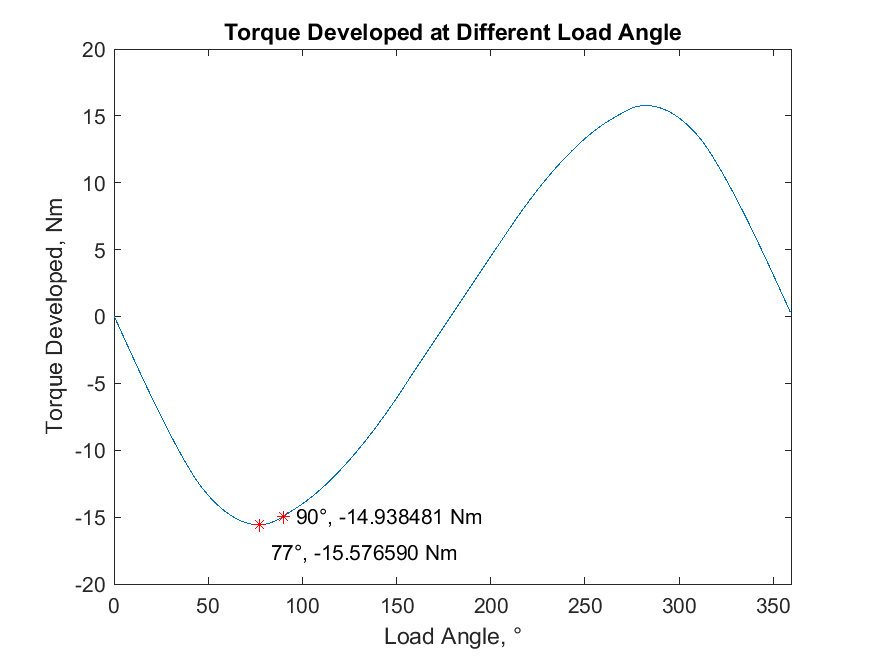
\includegraphics[width=1\linewidth]{img/task_3.png}
    \caption{Torque Developed at Different Load Angles}
    \label{fig:task-3}
\end{figure}

\begin{figure}[H]
    \centering
    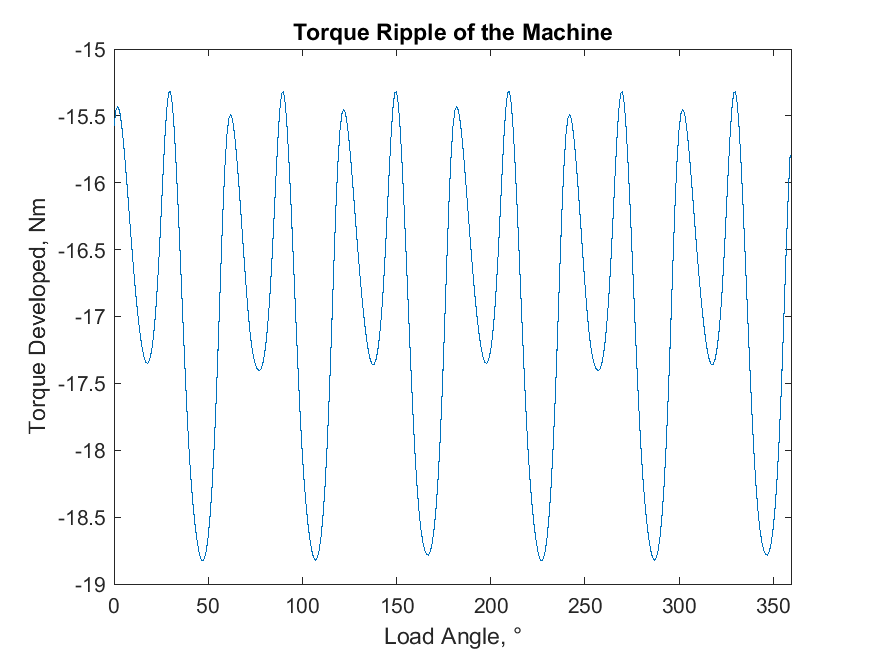
\includegraphics[width=1\linewidth]{img/task_3_ripple.png}
    \caption{Torque Ripple of the Machine}
    \label{fig:task-3-ripple}
\end{figure}

\subsection{Analysis}

Even though the theoretical peak torque should be at $\ang{90}$ load angle, the simulated value is slightly different at $\ang{77}$. This is due to the non-linear B-H curve of the stator and rotor materials.

The period of the torque ripple is $\ang{30}$ (12 pulsations per electrical revolution). This is twice the period of the cogging torque. It is twice as long because the electrical speed is two times faster than the mechanical speed (2 electrical rotation per mechanical rotation). This is also why the rotor is rotated at half the angle instead of rotating at the same speed.

The magnitude of the torque ripple is $3.513$ Nm. The mean torque of the machine is $16.9430$ Nm.

\section{Task 4}

The fourth task is to measure the magnetic flux density at various spots on the motor. Three main parts were measured, they are at the permanent magnet, the centre of the stator teeth and at the stator yoke. The magnetic flux density at various multiples of rated current is simulated. A current from 0 to 10 times the rated current is tested with an increment of 1.

\subsection{Methodology}

The magnetic flux density is measured at a load angle and rotor angle that generates the maximum torque. This is to ensure the magnetic field generated by the permanent magnet does not oppose and attenuate the field generated by the windings. The circuit property currents are modified with the multiplier.

For an accurate measurement, a simple simulation to compare where the highest flux density induced. The spot with the highest flux density in the teeth and yoke were noted. For the permanent magnet, the centre point of the magnet were used for the measurement. The measurement spots are shown in figure \ref{fig:task-4-measurement}.

\begin{figure}[h]
    \centering
    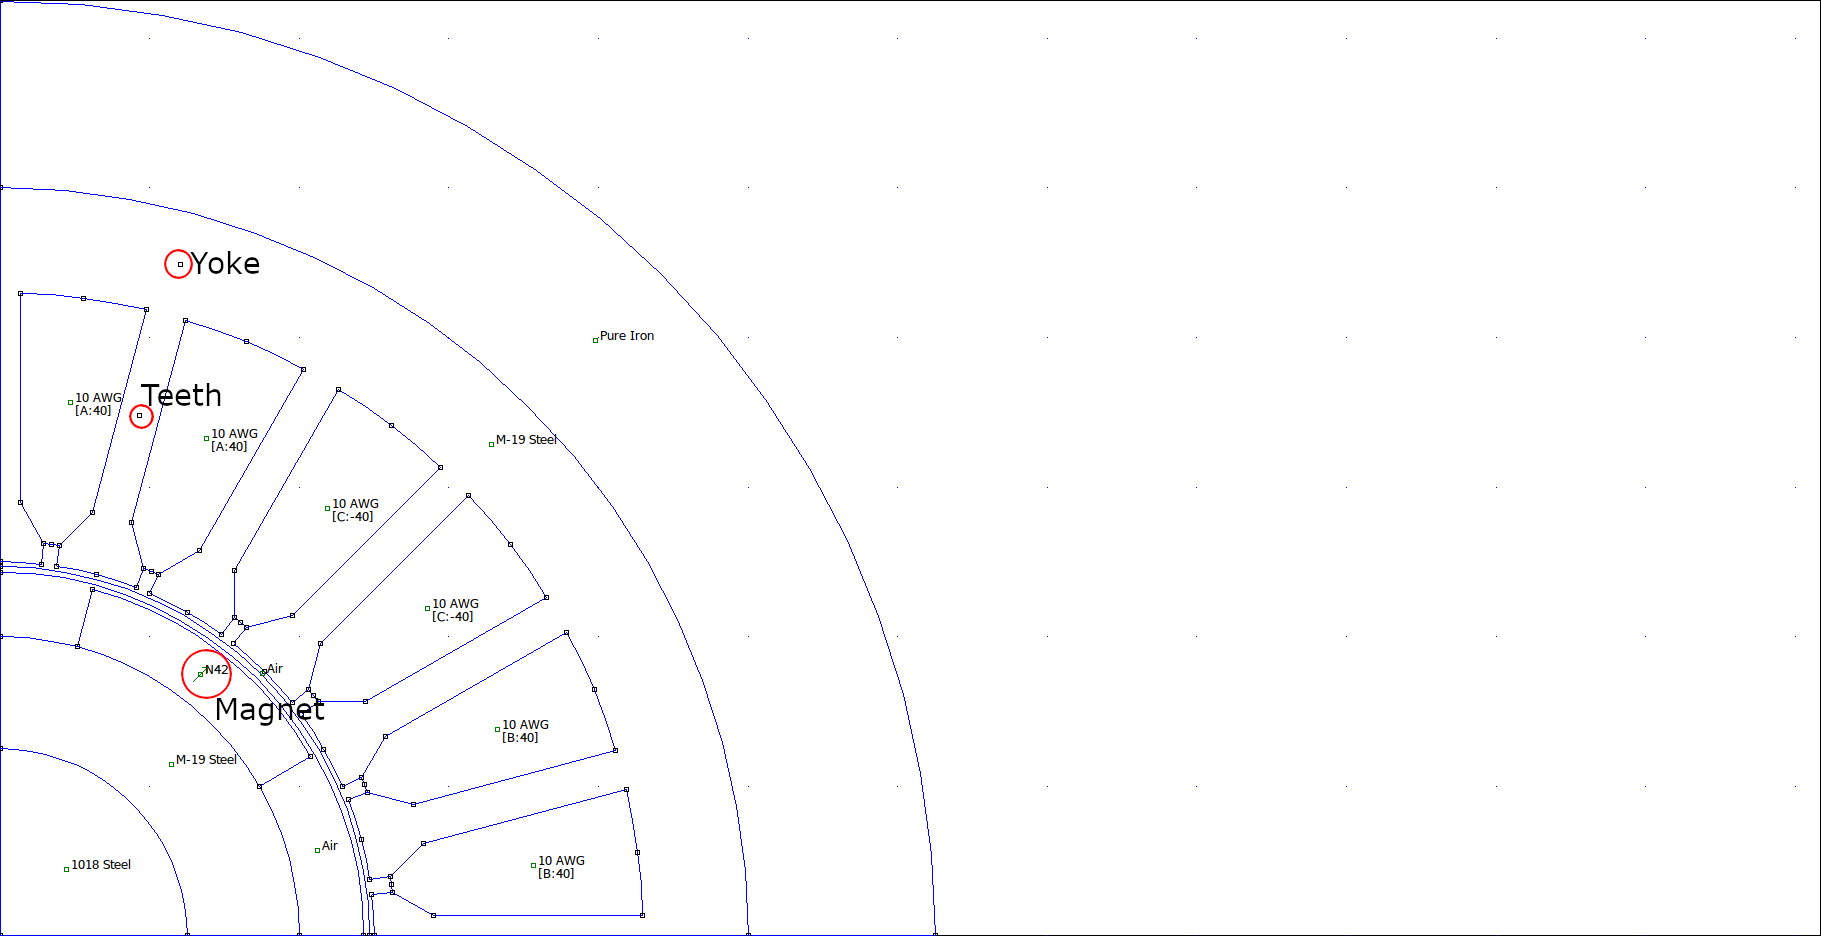
\includegraphics[width=1\linewidth]{img/task_4_measurement_edited.png}
    \caption{Measurement Location for Magnetic Flux Density}
    \label{fig:task-4-measurement}
\end{figure}

FEMM provides a MATLAB interface for getting the magnetic field at a point. The \lstinline{mi_getb}, measures the magnetic field density at a given x and y location. This interface returns two values, they are the magnetic flux density on the x ($B_{x}$) and y ($B_{y}$) plane. The total magnetic flux density ($B$) can be found using equation \ref{eq:mag}.

\begin{equation}\label{eq:mag}
    B = \sqrt{B_{x}^{2} + B_{y}^{2}}
\end{equation}

\subsection{Results}

\begin{figure}[h]
    \centering
    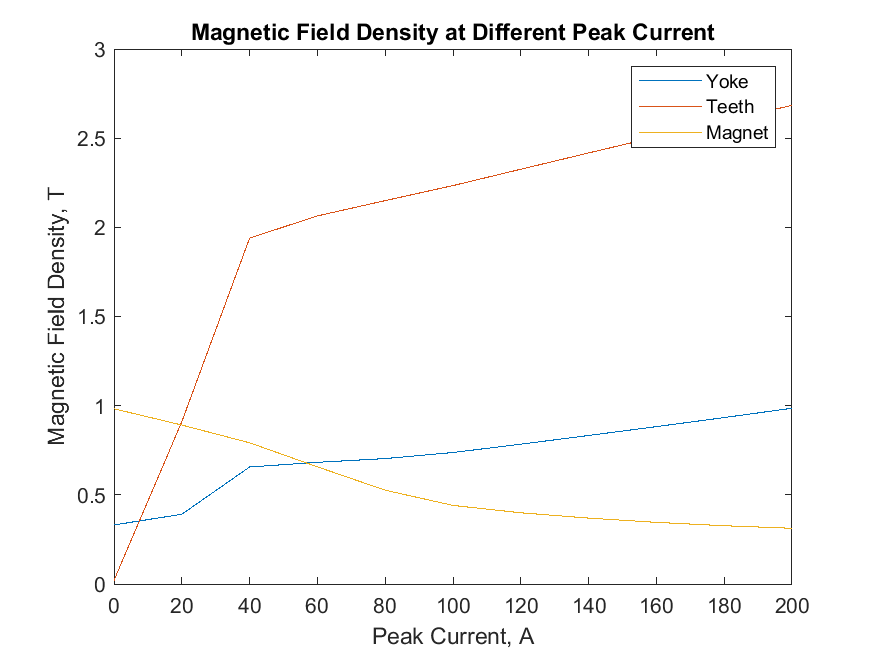
\includegraphics[width=1\linewidth]{img/task_4.png}
    \caption{Magnetic Flux Density at Different Peak Currents}
    \label{fig:task-4}
\end{figure}

\subsection{Analysis} \label{task-4-analysis}

At the teeth, the magnetic flux density increases at a high rate, from 0 to 4 times the rated current. This coincides with the rapid increase in current. However, the magnetic flux density change slows down due to the saturation in the teeth. The amount of flux density a material has is related to the B-H curve of the material. Once the magnetic flux intensity reaches a certain point, the flux density stop increasing as much.

The magnetic flux density at the yoke increases at a fairly constant rate. This is due to the larger cross-sectional area in the yoke. The generated magnetic flux intensity is spread out in a larger area, causing the stator to not saturate.

The magnetic flux density at the magnet decreases as the current increases. This is caused by the opposing magnetic field generated by the windings (direction of magnetic field). The opposing field cancels the magnetic field at the magnet, reducing the magnetic field density in the magnet.

\section{Task 5}

This task is similar to task 4. Instead of the magnetic flux density, the mean torque developed at different load current is explored. The mean torque is the mean of the torque developed at different rotor angles.

\subsection{Methodology}

The torque ripple at different load current is collected by varying the load angle and rotor angle (see \ref{task-3-method}). For each iteration of different load current, the mean of the torque ripple is recorded.

\subsection{Results}

\begin{figure}[H]
    \centering
    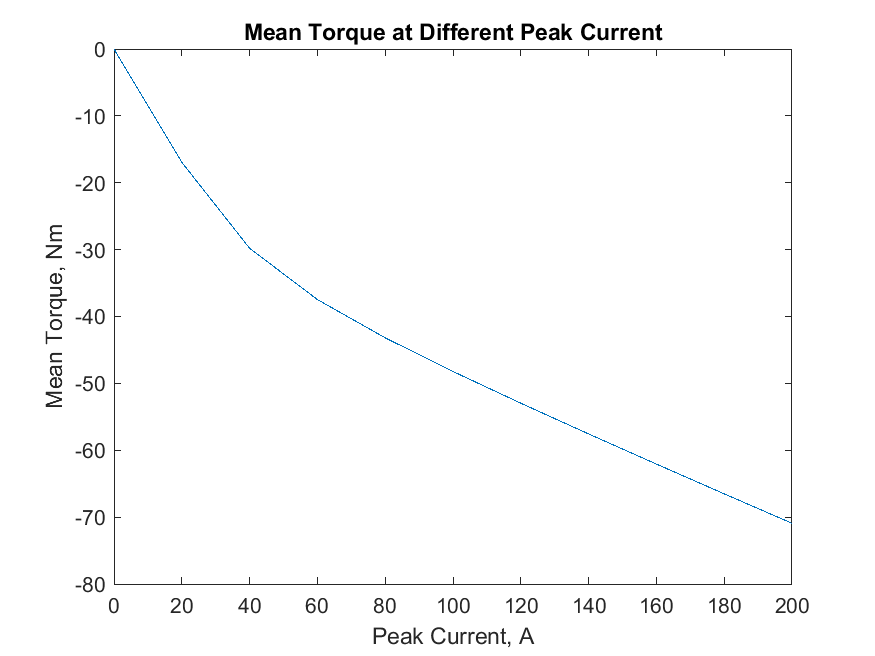
\includegraphics[width=1\linewidth]{img/task_5.png}
    \caption{Enter Caption}
    \label{fig:enter-label}
\end{figure}

\subsection{Analysis}

The mean torque developed increases by a lot as the load current increases. However, the rate of increase slows down with each increase of current. This is expected as the results of \ref{task-4-analysis} shows the saturation of the stator at high currents. The saturated stator have less magnetic field density, which results in lower torque developed in a rotor.

\section{Task 6}

\begin{table}[H]
    \centering
    \begin{tabular}{|l l | l l|}
         \hline
         AMPS& 14.142& VOLTS& 415\\
         \hline
         FREQUENCY& 50& &\\
         \hline
         TORQUE DEVELOPED& 16.9430& LOAD ANGLE& 77\\
         \hline
         RPM& 1500& HP& 3.5690\\
         \hline
         PHASE& 3& POLES& 4P\\
%         \hline
%         COGGING TORQUE FREQ& 24& COGGING TORQUE MAG& 0.3068\\
%         \hline
%         BACK EMF& 113.1587& MACHINE CONSTANT& 0.7204\\
%         \hline
%         RIPPLE FREQ& 12& RIPPLE MAG& 3.5130\\
         \hline
    \end{tabular}
    \caption{Nameplate for the Machine}
    \label{tab:nameplate}
\end{table}

\end{document}
